\documentclass[]{article}
%opening
\title{Writeup Document}
\author{Alex Miller}
\addtolength{\oddsidemargin}{-.875in}
\addtolength{\evensidemargin}{-.875in}
\addtolength{\textwidth}{1.75in}
\addtolength{\topmargin}{-.875in}
\addtolength{\textheight}{1.75in}
\setcounter{secnumdepth}{0}
\usepackage{cancel}
\usepackage{amssymb}
\usepackage{amsmath}
\usepackage{hyperref}
\usepackage{graphicx}
\graphicspath{ {./} }
\usepackage[ruled,vlined, linesnumbered]{algorithm2e}
\DontPrintSemicolon


\begin{document}
\maketitle

\section{Changes}
\subsection{Changes to the design}
The following addresses changes I have made to my projects design, broken down by module:
\begin{itemize}
	\item Top level modules (serial.c, parallel.c, my\_test\_serial.c, my\_test\_parallel.c) -- These files will take in the same inputs and utilize the same basic functionality as previously described in my design document. The following aspects will be modified
	
	\textbf{serial.c and parallel.c}
	\begin{itemize}
		\item I originally proposed to perform the lock tests required by the assignment by comparing the runtimes for a serial counter as opposed to a parallel counter using my lock implementations. In order to implement comparable behavior between my serial and parallel counters, I thought that the serial counter should increment an integer within a single for-loop B times, while the parallel counter should launch N threads which each increment a shared counter B / N times.
		\\\\
		This Design went under two key revisions. The first was that the parallel counter was redesigned such that each thread, within an infinite while loop, acquires the lock, and checks whether a volatile shared counter is less than B; if so, the given thread increments the shared counter, unlocks, and goes to the top of the while loop. Otherwise the thread unlocks and returns. 
		The parallel counter now also returns a long, instead of an int type.
		The motivation for this change was so that the critical section of the parallel counters would look more like that of the for loop described in the serial counter. Like a for loop, it involves checking whether an integer is less than B, and, if so, incrementing that integer. Otherwise each thread would have to maintain a shared counter which they would have to read and write each cycle, on top of incrementing the counter.
		\\\\
		The second change was to the serial counter. Like the parallel counter, it now returns a long. It initially was designed to check and increment a integer without the volatile attribute. However, when this approach was tested, the serial counter was able to output near-0 run times. This was probably due to compiler optimization. To mitigate this, as well as make the serial counter more like the parallel counter, the integer the serial counter uses has the volatile type, which stops the compiler from being able to make complicating optimizations.
	\end{itemize}
	\textbf{my\_test\_serial.c and my\_test\_parallel.c}
	\begin{itemize}
		\item $usleep()$ actually sleeps programs in microseconds, so instead, both my serial and parallel sleepers make their threads sleep for $usleep(t * 1000)$ microseconds at a time.
		
		Additionally, I also modified the functionality of the parallel sleeper in much the same way as I modified the parallel counter. Rather than each of the N threads sleeping for $usleep(t * 1000)$ microseconds $B / (t * n)$ times, each thread, within an infinite while loop, acquires the lock, and checks whether a  volatile shared counter is less than B; if so, the given thread increments the shared counter by t,  calls $usleep(t * 1000)$, unlocks, and goes to the top of the while loop. Otherwise the thread unlocks and returns.
		This behavior mimics that of the serial sleeper, which has to utilize a for-loop, without necessitating the use of extra confounding variables. The serial sleeper utilizes a volatile long to monitor progress in order to equalize performance even further.
	\end{itemize}
	\item Algorithm implementation level
	\\\\
	\textbf{lock.c}
	\begin{itemize}
		\item  I more thoroughly defined as well as changed the structure of my locking interface. I ended up defining my $lock\_methods$ struct under the struct name $lock_t$. The struct has the following attributes:
		\begin{itemize}
			\item char type : a reference to a lock type, as specified by input
			
			\item int B : The number threads should count/sleep to. I included this integer in order to make passing arguments to the threads as easy as passing them a pointer to this struct.
			
			
			\item int t : This integer is used in the sleeper function. 
			
			\item volatile long counter : The counter the threads share and increment.
			
			\item void *l : a pointer to a lock object; this pointer is passed to the initialization, lock, and unlock functions.
			
			\item void (*init\_thread)(void *) : This function initializes any thread specific structures required by a lock. It should be called before a thread acquires the lock the first time.
			
			\item void (*lock)(void *) : a pointer to the lock's lock function; it should be called on the void *l (which points to the initialized lock) in order to acquire the lock. 
			
			\item void (*unlock)(void *) : a pointer to the lock's unlock function; it should be called on the void *l (which points to the initialized lock) in order to release the lock. 
		\end{itemize}
		\item I defined an $init\_thread()$ function for each lock; this method simply returns for all locks except the MCS lock, which requires thread specific QNode structs, as defined in the textbook.
	\end{itemize}
	\item Testing script (test\_script.sh)
	\begin{itemize}
		\item Now that threads don't increment a shared counter an equal number of times, but instead perform an undetermined amount with the use of value checking, the $B$ values used in these tests no longer have to be multiples of $N$. Furthermore, $B = 1120$ did not seem sufficiently large enough to mitigate the effects of variation. Therefore, for all counter tests $B = 10000$ instead.
	\end{itemize}
\end{itemize}

\subsection{Changes to Test plan:}
I have not made any changes to my test plan. I want only to remark here that by only inferring the correctness of my locks through the output of the shared counter, we can only infer that all of our locks satisfy mutual exclusions. This does not prove that our FCFS lock implementations preserve FCFS ordering. However, as that would require time developing an additional testing structure, I am choosing not to implement that here.

\section{Results}
The raw performance data for the Idle Lock Overhead, Lock Scaling, and Proprietary tests are stored in a folder called $HW3a/hw3a/exp\_data$. This folder contains the .csv files that describe performance data for a given experiment. This data was collected by running implementations for given number of trials, calculating measurements per trial, and taking median values. As such there is no other collected data other than median speedup and throughput. That data was not recorded as it did not serve the purpose of analysis and would've have complicated my data storage scheme.
\\\\
As per how many trials I utilized; for experiments utilizing uniform and constant packets, I used 5 trials. I though this was sufficient for our counter tests, and would have to suffice for my sleeper tests, as those take quite while (at least 3 seconds each).
\\\\
I took this data and plotted it using the script analyze.py. These graphs are stored in the folder $HW3a/Docs/graphs$. I will display these graphs below:

\subsection{Experiment 1: Idle Lock Overhead}
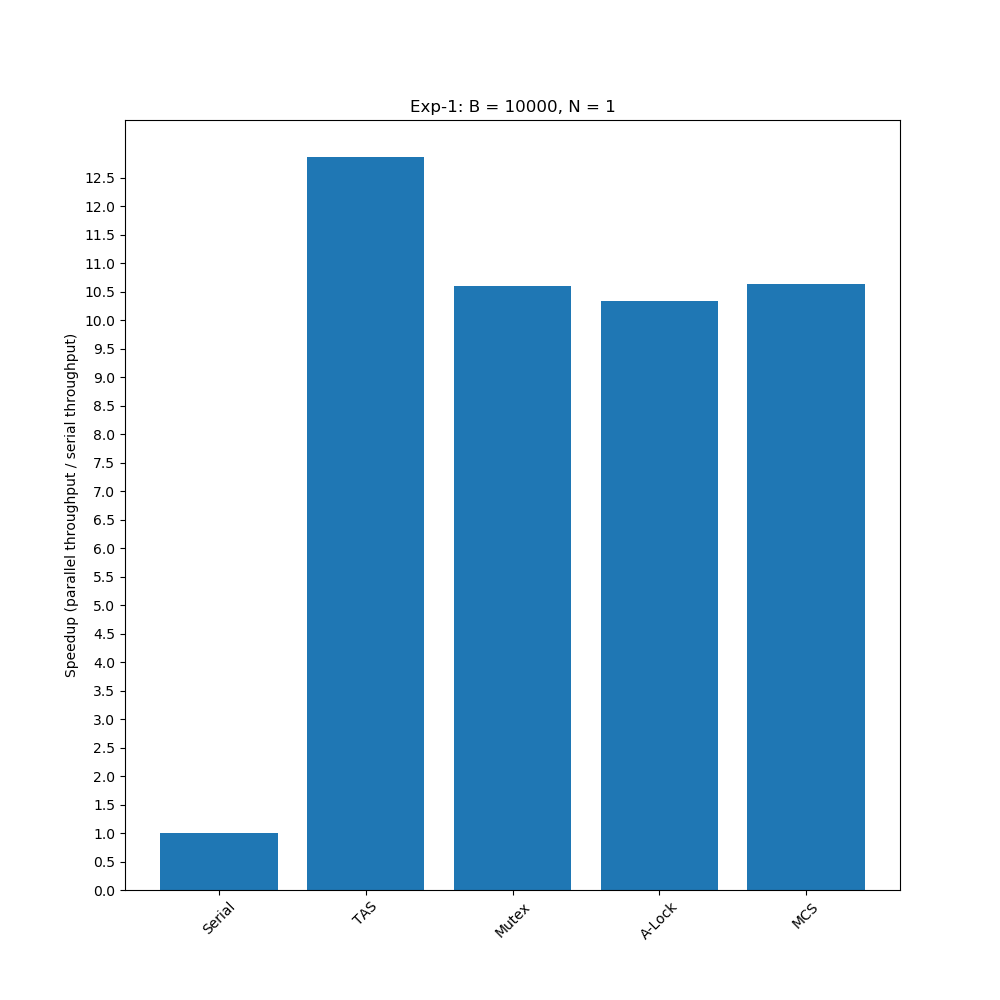
\includegraphics[scale=0.5]{graphs/exp1.png}\\
\subsection{Experiment 2: Lock Scaling}
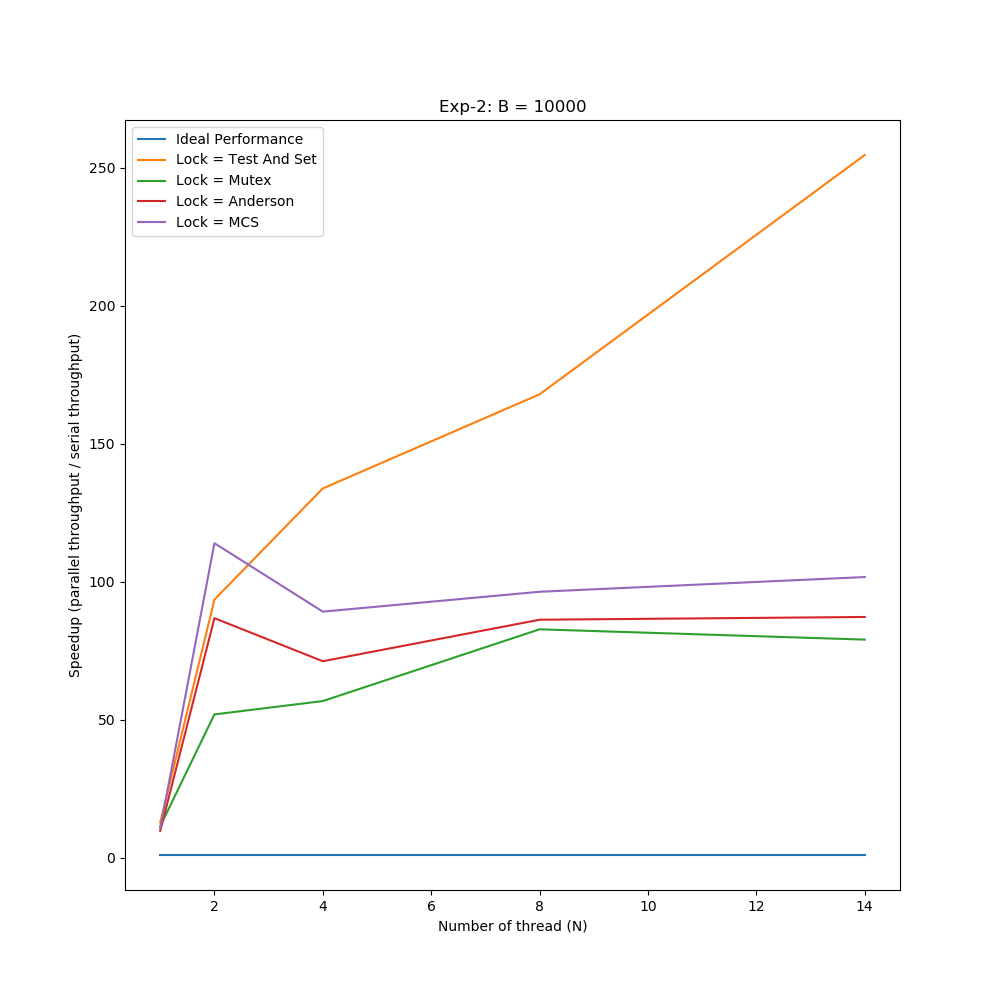
\includegraphics[scale=0.5]{graphs/exp2.png}\\
\subsection{Experiment 3: My Test}
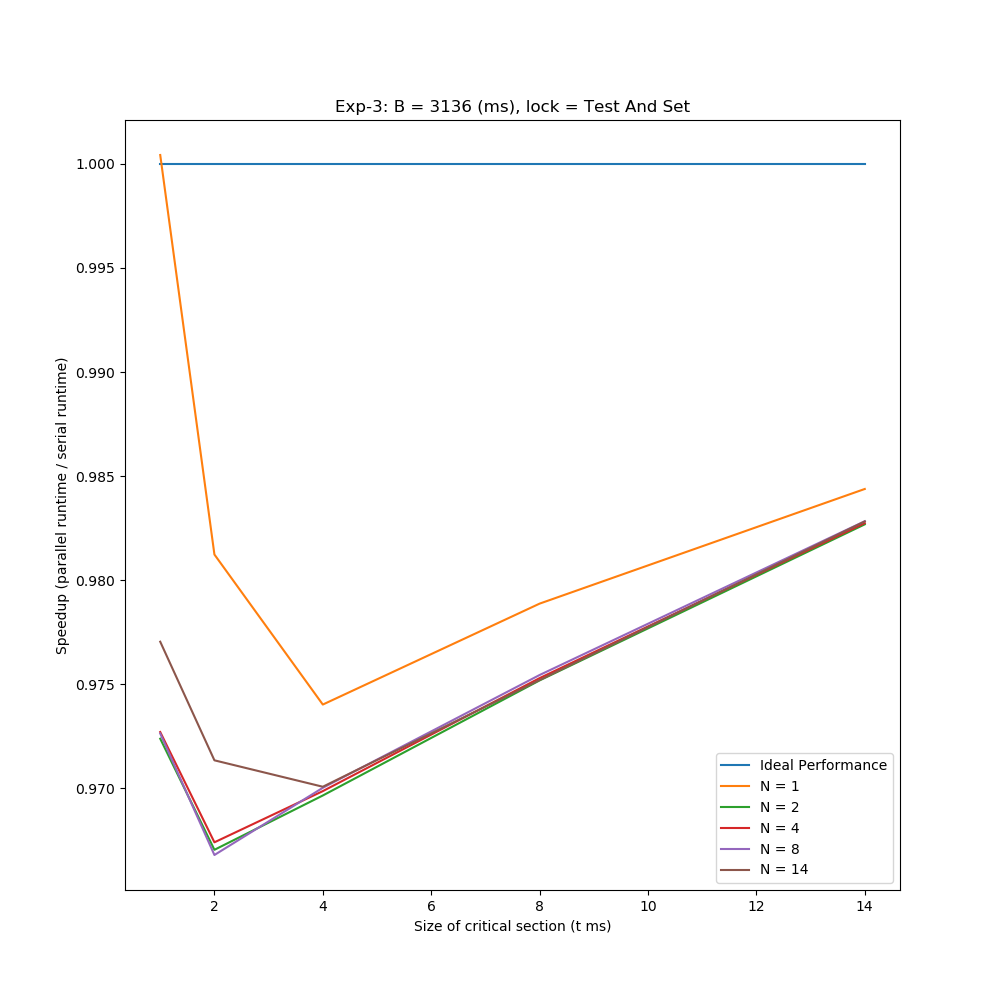
\includegraphics[scale=0.5]{graphs/exp3_t.png}\\
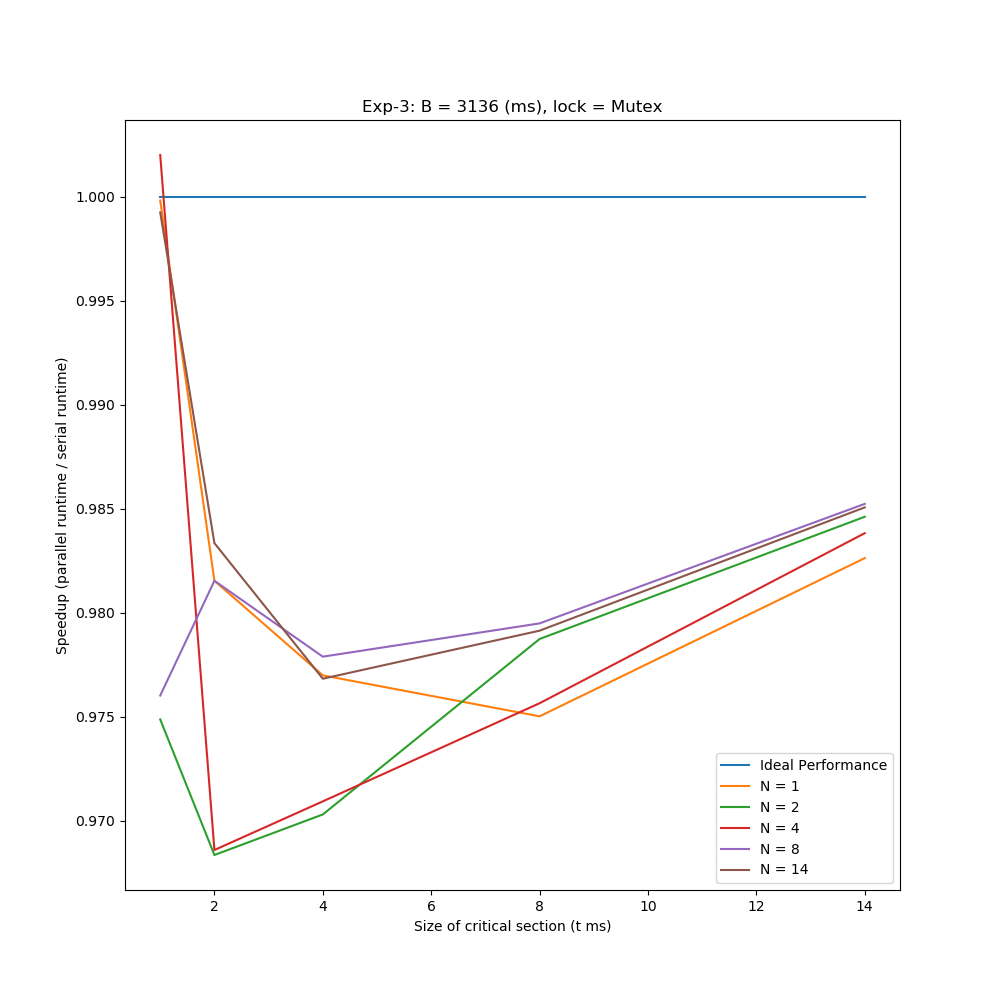
\includegraphics[scale=0.5]{graphs/exp3_p.png}\\
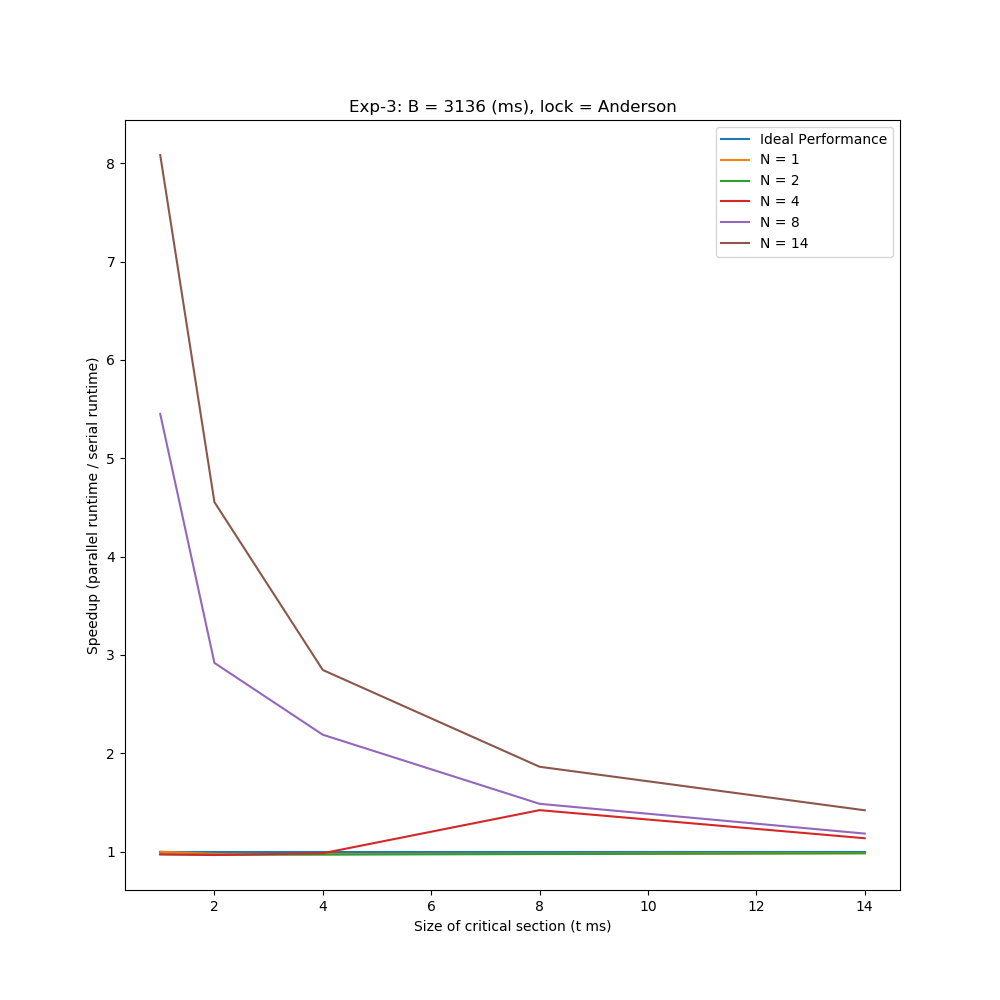
\includegraphics[scale=0.5]{graphs/exp3_a.png}\\
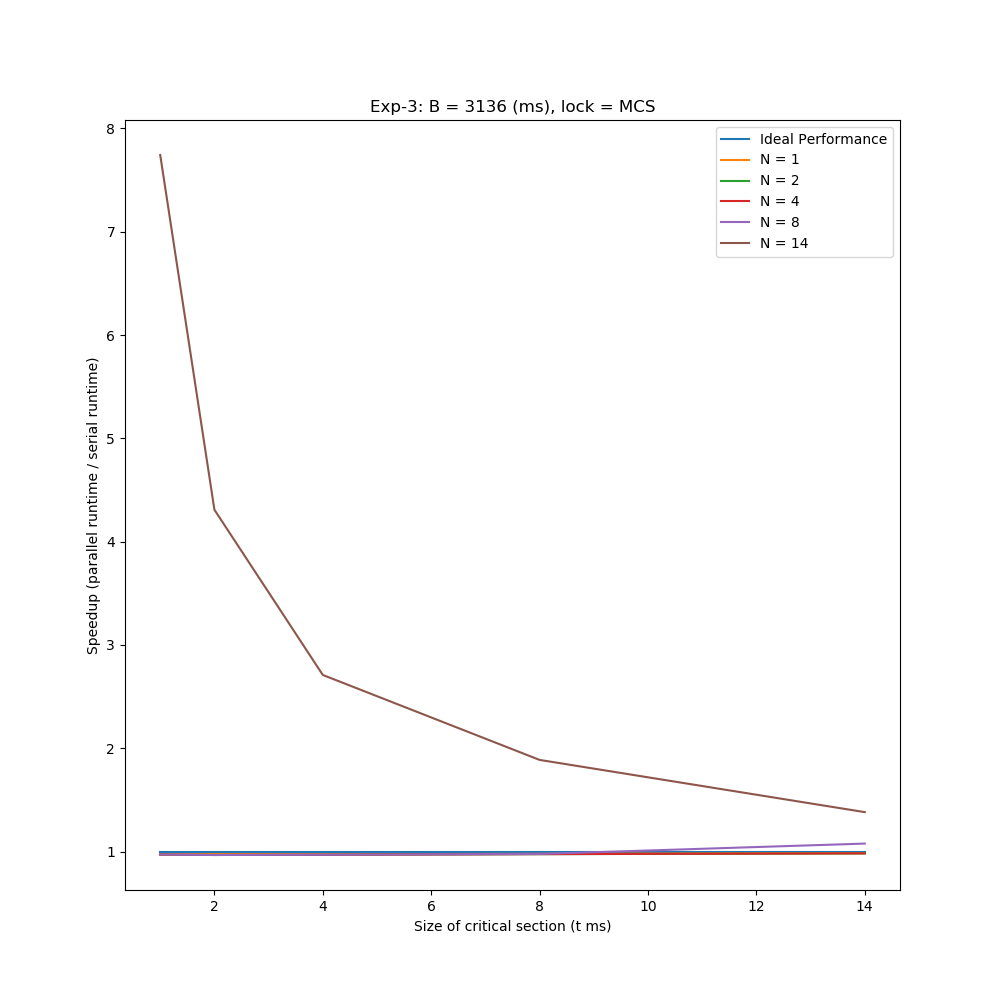
\includegraphics[scale=0.5]{graphs/exp3_m.png}\\

\section{Analysis}\subsection{Idle Lock Overhead}
The purpose of this test is to test lock performance in the complete absence of contention. Therefore, I hypothesized that locks would perform better in proportion to the relative simplicity of their lock and unlock methods. Locking algorithms with simpler lock and unlock methods will experience greater throughput, and be more likely to approach ideal, serial performance.
\\
Therefore, I expected to see the best performance from our Test and Set lock, followed by the Mutex lock, then our MCS lock, and lastly our Anderson's Array lock. 
\\\\
As the data shows, this was not the case. The Test and Set lock had the most overhead of any other lock, taking 21\% more time to complete its counter operation than the next slowest lock, the MCS lock. The MCS lock in turn had comparable performance with both the Mutex lock and the Anderson lock,though it took 0.3\% and 2.9\% more time to complete its counting operations, as respectively compared to those other locks.
\\
In order of least to most overhead, the data demonstrates that the Anderson lock had the least, followed by the Mutex, then MCS, then Test and Set Locks.
\\\\
The first intriguing aspect of this data is the that parallel counting operations with any lock and a single counting thread should take an order of magnitude longer to complete than our serial counter. I personally hardly expected to see up to 12X slowdown for the Test and Set lock. On my own machine, I recorded slowdown more on the order of 4 to 5X across different locking algorithms. This outcome can perhaps be the result of resource contention on the slurm machine at testing time, as increased load would slow performance. However, as both serial and parallel counters only utilize one thread under this test, it is not clear why the serial counter should run so much faster than our parallel implementations. Perhaps slowdown only started to occur after the testing script had already collected data on serial counter runtimes. 
\\
Another confounding factor could be the correctness of my parallel counter implementation; there may be something about performing my counting operations within a while loop, as opposed to a for loop, that negatively impacts performance.
\\\\
The second intriguing aspect of this data are the performance orderings described above. As I stated above, I did not expect the Test and Set lock to perform so badly, nor did I expect the MCS and Anderson locks to perform on par with the Mutex lock, especially since those formerly mentioned locks both utilize thread keys and one uses malloc(), both of which are expensive system calls, while the Mutex lock should merely call an atomic increment in the absence of contention.
\\
Perhaps the greater than expected run times for my Mutex and Test and Set locks are due to programming errors or confounding structures. The first explanation seems unlikely as these locks are sufficiently simple. The second might explain why I did not see better performance out of the Mutex lock; including it in the Locking interface described above requires wrapping its functions, possibly increasing lock and unlock complexity. Regardless, these increased run times are plausibly not intrinsic to lock performance, as these locks normally only suffer in the presence of contention between threads, which was notably absent in this test; the Test and Set lock threads should experience increasing numbers of cache invalidation as a function of increased contention, and the Mutex lock should likewise experience increased instances of thread backoff. Therefore, perhaps system overuse may be causing the slowdowns described in our data.
\\\\
Leaving the Mutex and Test and Set lock aside, the Anderson and MCS locks also did not perform as expected, with the Anderson lock taking less overhead than the MCS lock. However, this makes sense considering that each thread utilizing the parallel counter with the MCS lock has to call malloc() once, while threads using the Anderson lock do not. It is also notable that, even in the absence of contention, the MCS lock has to utilize atomic operations, which may impact performance, while the Anderson lock does not, which goes further to explain why the Anderson lock should experience less total overhead.
\subsection{Lock Scaling}
The purpose of this test is to test lock performance in the presence of contention from multiple threads trying to enter a shared critical section. Therefore, I predicted that locks will perform better in proportion to their ability to handle contention. Performance would vary, then, as a function of $N$; I thought that locks that are better at handling contention would experience less slowdown than locks that are worse at it. Additionally, I expected all parallel implementations to experience greater slowdown for greater values of $N$; since more threads merely implies greater contention and not increased parallelism, we should expect more threads to worsen performance for parallel lock tests.
\\
Therefore, I expected, in terms of relative performance in the face of larger values of $n$, that our MCS lock should perform best, followed by our Anderson's Array lock, then the Mutex lock, and finally our Test and Set lock.
\\\\
As the data shows, this contention was not entirely correct or consistent for all values of $N$. Notably, the MCS lock counter actually performed the worst of all locks for $N = 2$ threads, taking 21.8\% longer to complete than the Test and Set lock counter, 31.2\% longer than the Anderson Lock counter, and 119.4\% longer than the Mutex lock counter. However, for all $N > 2$, the data demonstrates a consistent total ordering, with the Test and Set lock counter performing the worst, followed by the MCS lock counter, then the Anderson lock counter, and lastly the Mutex lock counter, which performed the best. For $N = 14$, the Test and Set lock counter took 150.3\% to complete than the MCS lock counter, which in turn took 16.5\% longer to complete than the Anderson lock counter, which in turn took 10.3\% longer to complete than the Mutex lock counter.
The data therefore supports the following total ordering of lock performance for greater number of threads: in the presence of increased contention, the Mutex Lock performs best, followed by the Anderson lock, followed by the MCS lock, and finally the Test and Set lock.
\\\\
Though our data does not support our original hypothesis on total ordering, these observations do somewhat confirm my suspicion that MCS and Anderson's Array lock should showcase \textit{similar} performance, as they utilize the same principle of spinning on local cached memory, which cuts down on cache invalidation and misses, as potentially experienced by the Test and Set lock. Consider the following comparisons in runtime for varying values of $N$:
\begin{itemize}
	\item For $N = 2$, the MCS lock counter took 31.2\% longer to complete than the Anderson Lock counter
	\item For $N = 4$, the MCS lock counter took 25.2\% longer to complete than the Anderson Lock counter
	\item For $N = 8$, the MCS lock counter took 11.7\% longer to complete than the Anderson Lock counter
	\item For $N = 14$, the MCS lock counter took 16.5\% longer to complete than the Anderson Lock counter
\end{itemize}
The MCS lock performs at similar, if not consistently slowed, levels than the Anderson lock; this is also attested to by the similar shapes of these locks' data curves.
\\
That, between these two locks, I did not observe the strict ordering that I hypothesized is probably due to the increased overhead of the MCS lock over the Anderson lock, as observed and discussed above.
\\\\
The data does support my hypothesis that the Test and Set lock should demonstrate the worst performance of the group in the presence of increasing levels of contention. As stated in my design document, this is due to the abundance of cache misses resultant of multiple threads repeatedly invalidating thread-local copies of the shared $state$ boolean.
\\\\
However, my hypothesis that the Mutex lock performance should suffer in the presence of increased contention, as compared to the Anderson and MCS locks, was wholly wrong. Rather, it seems that, even though the Mutex lock spins on local memory of a shared integer value, which is vulnerable to cache invalidation, it's performance is redeemed by its employment of backoff. This indicates that the memory techniques used in the Anderson and MCS locks aren't alone sufficient to develop well-performing locks. Though backoff should invalidate any FCFS property we may wish to include in our locking implementations, it offers itself as a significantly useful way to artificially reduce lock contention and therefore increase lock performance.
\\\\
The data does somewhat support my hypothesis that all parallel implementations of our counter utilizing locks should experience greater slowdown for greater values of $N$. This is obviously true of our Test and Set lock, which reported increased slowdown for each successive value of $N$. This relationship is more muddled for our other locks. The Anderson and Mutex locks observed initial spikes in run time for $N = 2$, followed by more level, if not slightly increasing, curves. The Mutex lock observed a 4.7\% decrease in run time between $N = 8$ and $N = 14$. This may be a system runtime aberration. More testing, possibly for larger values of $N$, is needed to determine if this stated relationship between slowdown and $N$ is well supported. It may well be that certain locks demonstrate a certain limit to possible slowdown as $N$ increases to $\infty$
\subsection{My Test}
The purpose of this test if to determine the effect of critical section size on lock performance. In general, I expected less relative slowdown of our parallel implementations over our serial implementation for larger critical sections (larger values of $T$), as the increased necessary compute times in the critical section should otherwise cancel out increased waiting time to acquire a lock due to contention. That being said, I also expected to see more relative slowdown for larger values of $N$; this reflects our previous hypothesis that increased contention for a lock should increase slowdown in all cases, which was somewhat supported by our analysis of the prior experiment.
\\\\
In lieu of a hypothesis on relative performance between locks, I expected there to be a point for all locking algorithms at which the size of the critical section outweighs slowdown due to contention. Therefore, for a large enough value of $T$, I expected all locks to showcase near-ideal performance for all values of $N$.
\\\\
%Address observed speedup...%
The data seriously complicated my prior assumptions and understanding. For at one least data point (comprising a cross product of $N$ and $T$), each lock demonstrated speedup in its parallel sleeper over the serial sleeper. Many individual curves in this test are actually consistently sped-up for all values of $T$. For example, for the sleeper test of the Anderson lock where $N = 2$, no individual test took longer to complete than the comparable serial sleeper test; for $N = 2, T =1$, the Anderson lock sleeper ran 0.02754\% faster than the serial sleep and for $N =2, T = 14$, 0.01724\% faster.
\\
Therefore, my assumption that these tests should only exhibit slowdown was largely mistaken. This is an odd result in any case, considering that in our test of lock overhead, no locking algorithm was able to complete its parallel counter within an order of magnitude of the serial counter. Perhaps this is explained by the fact that the critical section may actually be entered more readily in the parallel sleeper than in the serial sleeper, due multiple threads trying to enter the critical section. But if this was true, we wouldn't experience such speedup for $N = 1$, or the slowdown in the last experiment.
\\
Perhaps the presence of this speedup is due to the reality of run time aberrations in the system. In this case, the data could possibly be improved by running the same tests for greater values of $B$; doing so would mitigate potential run time variations. However, as $B$ is a total program sleep time, increasing it's value would proportionally increase the runtime of our tests, which is undesirable considering the shared nature of the testing environment. Perhaps more testing is needed for larger values of $B$.
\\\\
Despite this complication, our original hypothesis that sleeper performance for various values of $N$ should converge for large enough values of $T$ conforms to our performance data for the MCS lock and Anderson lock. For example, in the case of the Anderson lock, the run-times for $N = 1,2,4,8,14$ converged to ideal performance for large enough values of $T$. For $T = 1$, the $N = 14$ trial took 700.1\% longer to return than the $N = 1$ trial, while, For $T = 14$, the $N = 14$ trial only took 44.2\% longer to return than the $N = 1$ trial. Likewise,  in the case of the MCS  lock, the run-times for $N = 1,2,4,8,14$ converged to ideal performance for large enough values of $T$. For $T = 1$, the $N = 14$ trial took 686.4\% longer to return than the $N = 1$ trial, while, For $T = 14$, the $N = 14$ trial only took 40.5\% longer to return than the $N = 1$ trial. 
\\
Likewise, for these lock tests, the data also conforms to my expectation to see more relative slowdown between the sleeper test for a given lock for larger values of $n$. The curves for the Anderson lock sleeper tests demonstrate this the best, as the value of the curves for $N = 4, 8, 14$ are strictly ordered so. This hypothesis is also supported slightly by the MCS data; its curve for $N = 14$ was strictly greater than all other curves for all other values of $N$.
\\\\
The most perplexing aspect of our data for this test was those curves for the Test and Set and Mutex locks. Not only did both of these locks consistently demonstrate speedup in their parallel sleepers in comparison to the serial sleeper, their tests' curves also exhibited local minimums for $T = 2$ or $4$ before converging on ideal performance for larger values of $T$. I thought that convergence towards ideal performance would occur as a function of thread contention being dwarfed by the size of the critical section. However, these results demonstrate that the size of the critical section mitigates inexplicable gains in performance experienced by these tests' locks. If anything, increasing size of the critical section, by making threads wait longer, increases the amount of cache invalidation that occur, causing closer to ideal performance through increased slowdown, as opposed to increase relative speedup.
\\
Overall, this data may confirm our hypothesis that that sleeper performance for various values of $N$ should converge for large enough values of $T$, if not in a way that confounds my understanding of why that happens. As to our hypothesis on curve ordering by the value of $N$, it is sorely mistaken to apply that idea here, as the curves presented in our graphs of Test and Set and Mutex data are intermixed. As to applying a quantitative understanding, that won't be attempted here, as I am not sure what more could be helpfully said about this confusingly confounded data set. Perhaps, as suggested before, more data is needed, with larger values of $B$.
\\\\
Before concluding, I would like to suggest a reason why we should observe different types of convergence on ideal performance, as elaborated above. Though we may not offer a good reason as to why any parallel counter should experience speedup over the serial counter, the relation between convergence to ideal performance and curve shape may reflect the type of lock being tested. For example, in the case of the Test and Set and Mutex locks, increased critical section size may force convergence to ideal performance through slowdown by virtue of increased contention and subsequent cache invalidation, as required by these locks designs. This would explain these locks greater relative slowdown in the presence of larger values of $T$. In the case of the Anderson and MCS locks, increased critical section size may force convergence to ideal performance because by mitigating the effects of contention. These locks don't experience the same slowdown as the others as they don't rely on local copies of shared state variables, which otherwise would cause cache invalidation and slowdown.
\end{document}
